\cleardoublepage %poner esta linea al inicio de cada capitulo

\chapter{Introducción}

La agricultura ha sido uno de los pilares más importantes tanto para el desarrollo de la sociedad como para su manutención, ya que es gracias a está, que los países pueden generar empleos y aumentar sus recursos económicos, sin embargo las tareas de agricultura pueden llegar a ser tediosas o muy pesadas para las personas, es por esto que con el avance tecnológico se ha buscado mejorar el sector agricultor no solo para facilitar a los agricultores las tareas que deben hacer, sino también permitir que el producto que están ofreciendo sea de mayor calidad, para garantizar que su comercialización tenga un mayor auge globalmente.
\\
La visión artificial se ha implementado en el sector agricultor para corregir las fallas humanas y garantizar que el producto mantenga siempre una buena calidad, ya que para poder exportar productos agrícolas estos deben estar bajo los requisitos de las normas INCONTEC.
\\
Este proyecto busca implementar mediante un proceso mecatrónico las técnicas de visión artificial para ayudar al crecimiento del sector papicultor en Colombia, el cual se ha visto afectado por los tratados de libre comercio establecidos por el gobierno nacional. 


\newpage
\section{Objetivos}

\subsection{Objetivo General}

Implementar un prototipo para la clasificación de características de calidad en los tubérculos de papa producidos en la región Andina de Colombia, mediante técnicas de visión por computadora.

\subsection{Objetivos Específicos}
\begin{enumerate}
	\item Identificar a través de técnicas de visión artificial los rasgos de calidad "y características físicas" que se encuentran en los tubérculos de papa. 
	\item Evaluar el desempeño del prototipo propuesto para realizar la clasificación de los tubérculos de papa bajo las categorias de tamaño grande mediana y pequeña establecidas por la norma NTC341. 
	\item Comparar la precisión del modelo propuesto con modelos similares de clasificación
\end{enumerate}

\section{Alcances y Limitaciones}

\subsection{Alcances}

Para la realización del proyecto se debe tener en cuenta que se enfocará en los tubérculos de papa tipo pastusa producidos en la región andina de Colombia, los cuales se deben encontrar lavados para llevar acabo un análisis más preciso, el análisis estará enfocado en identificar las características de calidad del producto predicho para ser comercializado. Ádemas de esto el prototipo propuesto será de ayuda únicamente en el desplazamiento del producto para su análisis. 

\subsection{Limitaciones}


El proyecto se encuentra limitado a los recursos de software y hardware (computacionales) con los que cuentan los integrantes del proyecto y las plataformas open sources que se le puedan sacar provecho para la implementación de los algoritmos que actualmente se encuentran en la literatura. Por otro lado se presentan limitaciones para la construcción del elemento por la contingencia sanitaria presentada hoy en día, los procesos de mecanizados como lo son el torno, la fresadora y la soldadura de la universidad se encuentran limitados por la contingencia.


\section{Justificación}
El presente proyecto implementará técnicas de visión artificial en el sector papicultor colombiano con el fin de comprobar la eficacia de la clasificación de calidad en los tubérculos de papa, ya que Actualmente, el cultivo de la papa constituye el eje fundamental de la economía del país en 283 municipios a nivel nacional, donde se involucran más de 90.000 familias principalmente en los departamentos de Boyacá, Cundinamarca, Antioquia y Nariño, los cuales concentran más del 85 \% de la producción \cite{referencia1}.
Actualmente el reto que enfrenta el sector es el aumento de la calidad del producto, el rendimiento en producción y en consecuencia, incrementar el consumo. Debido a que la producción de papa en Colombia aporta el 3.3 \% del Producto Interno Bruto (PIB) agropecuario, las siembras son de alrededor de 130 mil hectáreas y se cosechan cerca de 2,8 millones de toneladas, Además, en Colombia la producción de papa genera anualmente alrededor de 264.000 empleos, aproximadamente 75.000 son trabajos directos y alrededor de 189.000 son indirectos \cite{referencia2}
Así el presente trabajo permitirá mostrar los beneficios que trae la implementación de técnicas de visión artificial permitiendo un crecimiento al sector papicultor y aumentando la calidad del producto para que pueda ser comercializado tanto a nivel local como global.


\section{Descripción y formulación del problema}
La agricultura de Colombia es un componente fundamental en la economía del territorio, Juega un papel primordial en el desarrollo económico del país. Debido a que es la principal fuente de ingresos del área rural, hace un aporte relevante al desarrollo económico, la mitigación de la pobreza, y el desarrollo sustentable de Colombia. Uno de los sectores más   grandes en la agricultura colombiana es el sector papicultor, en Colombia se caracteriza por tener poco desarrollo tecnológico y buscar abastecer el consumo interno, sin mayor exploración en mercados internacionales. Frente a la coyuntura en la que se encuentra el sector gracias a los retos que trae consigo los acuerdos comerciales firmados por el gobierno nacional, el sector papicultor requiere urgentes transformaciones que permitan aumentar su competitividad y por ende lograr el crecimiento del sector.
Como consecuencia en los últimos años el sector agricultor de Colombia ha implementado herramientas tecnológicas que le permitan a los agricultores aumentar la calidad de sus productos y así poder competir tanto en el mercado local como en el global. Pensando en esto las diferentes técnicas de visión artificial han tenido un auge en la agricultura de precisión ayudando a clasificar productos basándose en sus diferentes características sin importar su clase, sin embargo, las técnicas de visión artificial no han sido aprovechadas para mejorar el sector papicultor colombiano.
El sector agricultor de Colombia ha implementado diferentes técnicas de visión artificial las cuales ayudan a clasificar los productos mediante las características que estos poseen, sin embargo no se ha implementado estas técnicas en la fase de almacenamiento de los tubérculos de papa, la cual es importante ya que en esta fase es donde se separan los tubérculos que cumplen las condiciones de calidad de los tubérculos que se encuentran defectuosos, ya que para la comercialización de este producto deben estar clasificados según la norma NTC 341.\\ 

¿Cómo se puede aumentar la eficiencia al clasificar los tubérculos de papa bajo la norma NTC341 mediante técnicas de visión artificial para su distribución comercial?\\

¿Qué tipo de proceso de clasificación permitirá agrupar los tubérculos de papa según sus características físicas y "patologías" mediante técnicas de visión artificial?	


\chapter{Estado del arte}

\section{MatLab.}
	El objetivo de los antecedentes es analizar y realizar una revisión literaria sobre lo  que  se  ha hecho  a  nivel  teórico  y  práctico  en  cuanto a  la visión artificial en agricultura de precisión.  Además,  determinar  cuáles son los aportes que éstos le puedan dar a este trabajo de investigación.\\
	
	Comenzando por la literatura con temática en el procesamiento de imágenes se tiene el artículo \cite{article3}, en donde se menciona que la implementación de MATLAB\textsuperscript{\textregistered} como una herramienta de procesamiento de imágenes, radica en su facilidad para realizar cambios a las imágenes, es por esto qué diseñó un sistema para la clasificación de objetos en base a su forma y color usando métodos de visión artificial en MATLAB\textsuperscript{\textregistered} con el uso de la librería \textit{ufm.dll} para capturar y procesar imágenes. El artículo \cite{inproceedings} presenta una investigación en dónde se consiguió calcular el tamaño de diferentes mangos estimando el área cubierta en una imagen binaria (imagen digital que tiene únicamente dos valores posibles para cada píxel) con base al número de píxeles, luego de ser procesadas las imágenes, se clasificaron implementando un algoritmo basado en \textit{fuzzy logic} teniendo en cuenta 5 variedades diferentes de mangos y como referencias el color de la cascara, tamaño, defectos superficiales, forma, firmeza, peso y olor.\\

\section{Artificial Neural Networks.}
	En cuanto a la clasificación, se deben usar técnicas de visión artificial y en primer lugar, se revisó literatura  acerca de ANN (\textit{Artificial Neural Networks}) como el articulo \cite{article2} en el Perú  aplicó visión artificial usando ANN como método de clasificación de las principales características extraídas de las frutas, que son derivadas del análisis de las superficies tanto en su contenido cromático como en la cantidad y distribución de defectos externos. De igual forma, en el trabajo \cite{Shrivastava2017}, presentaron un sistema de visión artificial que usa un enfoque de categorización simplificado con un elevado índice de exactitud. El propósito del sistema es clasificar los granos de trigo de las especies \textit{triticum aestivum} y \textit{triticum durum} según sus propiedades visuales usando una ANN del tipo MLP (\textit{Multilayer Perceptron}); las imágenes se obtienen por medio de una cámara que captura las propiedades de tamaño, color y textura de cada grano con el objeto de que sirvan de acceso al procedimiento de categorización. Otro trabajo es \cite{Singh2016}, quien propone el uso de redes neuronales BPNN (\textit{Back Propagation Artificial Neural Networks}) como método de clasificación y la descomposición mediante ondículas (Tipo especial de transformada matemática que representa una señal en términos de versiones trasladadas y dilatadas de una onda finita) para clasificar los granos de arroz. El modelo de clasificación implemento una red neuronal BPNN de cuatro capas la cual presento mejores resultados en comparación con otros métodos.\\
	
	Por último, usando el método de clasificación ANN, se tiene el artículo \cite{Przybyl2019} presenta un trabajo para garantizar la correcta clasificación de los productos y reducir las pérdidas durante su almacenamiento. La investigación abarca esfuerzos centrados en la evaluación sensorial de patatas con el análisis de imágenes por ordenador y la modelización neuronal ANN. El objetivo de este estudio fue desarrollar un método para asistir a la identificación de cualquiera de las variedades y la turgencia de los tubérculos de patata(Fenómeno que ocurre cuando una célula se dilata debido a la presión ejercida por los fluidos y por el contenido celular sobre las paredes de la célula) llevado a cabo sobre la base de los datos gráficos codificados en forma de imágenes digitales, obtenidos mediante algoritmos que interpretan los descriptores de imagen.\\

\section{Super Vector Machine.}
	Otro método de clasificación revisado en la literatura es el de SVM \textit{Super Vector Machine}), como el usado en el trabajo \cite{LIU201679}, en donde realizaron un proceso para analizar granos de arroz. El procedimiento usa 4 fuentes de luz para crear la sombra del grano en 4 direcciones; la diferencia en medio de las siluetas de los granos llenos y no llenos se evalúan por medio del estudio de imágenes y un clasificador SVM. El análisis se hace mediante el uso de imágenes RGB (Red-Green-Blue) de los granos con las siluetas, luego se segmentan por  desde la imagen binaria, para sustraer información como el sector del grano y de la sombra. En el documento \cite{CHUNG2016404} se menciona un método para clasificar plántulas (Embrión ya desarrollado como consecuencia de la germinación de una semilla) sanas e infectadas. Consiste en el análisis de imágenes mediante un escáner y el proceso de clasificación utilizando SVM, en donde se hace uso de dos clasificadores, el primero distingue entre las plantas sanas y contaminadas, por otra parte, el segundo mide los niveles de contaminación. En el trabajo \cite{PIRES201648} se propuso un método de detección automática de enfermedad en cultivos de soja, el cual se basa en descripciones locales conocido como el método BOV (Bag of Values) luego de escanear la hoja. Se obtuvo a través de los vectores de entrada una clasificación en dos categorías, enfermo y sano, a partir de un clasificador SVM. Y por último, en este tipo de clasificador, el documento \cite{SUN2014426} propone un sistema para analizar el porcentaje de granos en el arroz que se encuentran en condiciones para ser distribuidos. El algoritmo se encarga de la división de los granos de manera automática. Tras la segmentación, es viable obtener el número de granos presentes en la imagen y la información específica, la exactitud del procedimiento puede verse afectada si el germen no se extrae del todo por esa razón el sistema detecta la viable región de germen y estima esta información usando SVM.\\

\section{Otros métodos}
	En la literatura se encontraron artículos que usaban más de un método de clasificación, un ejemplo es \cite{LIU201682} que puso en práctica un método para controlar la población de pulgones (Familia de insectos hemípteros) en el trigo, usando los métodos SVM, el algoritmo MSER (\textit{Maximally Stable Extremal Regions}), y el HOG (\textit{Histogram of Gradients}).El uso de estos 3 métodos se conoce como SMH (Unión entre SVM, MSER y HOG, que se basa en el análisis de imágenes, tratadas a partir de unos parámetros con la finalidad de detectar la presencia y/o ausencia de pulgones, se hizo uso de este método a partir del color y la densidad de población. Al comparar este método con otros cinco comúnmente utilizados, los resultados presentaron un rendimiento superior en la identificación de pulgones. \\
	
	De igual manera, el artículo \cite{sobolu2020automatic} propone un algoritmo de clasificación automática de patatas. Se Realizó dos tipos de clasificación: una en función del tamaño de las patatas y otra en función de su calidad. La segmentación de las zonas defectuosas se hizo mediante métodos como \textit{global thresholding} para extraer \textit{morphological and statistical features} de las zonas segmentadas. Estas características se eligieron como entradas para los algoritmos de clasificación, en donde se usaron los métodos SVM, \textit{Decision  Tree} y LDA (\textit{Linear Discriminant Analysis}) implementados en MATLAB\textsuperscript{\textregistered} Classification Toolbox.Se llegó a la conclusión de que la SVM ha clasificado las patatas según su tamaño con una mayor tasa de éxito. En el caso de la clasificación por calidad, se recomienda el método LDA.\\
	
	Los anteriores son los métodos más comunes que se encontraron en la literatura investigada, sin embargo, hay unos métodos poco comunes como por ejemplo los presentados en el artículo \cite{article5} en donde se identificó objetos en movimiento mediante la ayuda de la visión artificial y la transmisión de datos a un brazo robótico implementando \textit{C++} y \textit{Open CV} usando el código de cadena (Actualmente el grupo de reconocimiento de patrones e inteligencia artificial aplicada) para calcular las características de los objetos por color y forma. También, el artículo \cite{7237209} que se usa para la detección automática, fue necesario hacer uso inicialmente de separar el fondo de la hoja, para este proceso se usó el algoritmo MCW (\textit{Marker-Controlled Watershed}), el SLIC (\textit{Simple Linear Iterative Clustering}) se utilizó para obtener las características presentadas por la enfermedad sobre la planta y por ultimo para la clasificación y textura se obtienen a través de GLCM (\textit{Gray Level Co-occurrence Matrix}), el modelo de clasificación fue el SVM, este método propuesto presento un mayor rendimiento.\\
	
	Y el último artículo revisado es el \cite{Barnes2010}, cuyo objetivo de  investigación es introducir un método automático de detección de manchas en imágenes digitales de patatas. El sistema desarrollado es entrenable, de modo que pueda trabajar con diferentes variedades de patatas y variaciones en las estaciones, condiciones de iluminación, etc. Otro objetivo, pensando en su posible implantación en entornos industriales, es permitir el procesamiento de imágenes en tiempo real, posiblemente mediante la construcción de \textit{Minimalist Boosted Classifier} que extraigan un subconjunto mínimo de todas las características que optimicen el rendimiento de la detección con el menor coste computacional posible.


\chapter{Marco Conceptual}

	\section{Agricultura de precisión} El término sobre el que se inspira la agricultura de precisión es utilizar la porción adecuada de insumos, en el instante correcto y en el sitio preciso. La agricultura de precisión (AP) implica la utilización de sistemas de posicionamiento universal (GPS) y de otros medios electrónicos para obtener datos del cultivo. Las tecnologías de la agricultura de precisión permiten saciar una de las exigencias de la agricultura actualizada: el funcionamiento óptimo de enormes extensiones. Se muestra como primordial virtud que la exploración de resultados de los ensayos se puede hacer por sectores diferentes en un mismo lote, y tal cual ajustar el desempeño diferencial en los mismos. La utilización de las tecnologías de la agricultura de precisión puede contribuir a mejorar los márgenes, por medio de un incremento del costo del rendimiento (cantidad o calidad), de una reducción en la proporción de insumos, o de los dos paralelamente.
	\\
	\section{Artificial Neural Networks} Las RNA son sistemas de procesamiento de la información cuya composición y manejo permanecen inspirados en las redes neuronales biológicas. Consisten en un enorme conjunto de recursos básicas de procesamiento denominados nodos o neuronas que permanecen organizados en capas. De esta forma, las RNA son sistemas adaptativos que aprenden de la vivencia, en otros términos, aprenden a realizar ciertas labores por medio de un entrenamiento con ejemplos ilustrativos.
	\\ 
	
	\section{Imagen Binaria} La binarización de una imagen se apoya en un proceso de reducción de la información de la misma, en la que únicamente persisten 2 valores: verdadero y falso. En el proceso y estudio de imagen, la binarización se emplea para dividir las zonas u objetos de interés en una imagen del resto. En otras ocasiones, una imagen binaria es sencillamente el resultado de una selección interactiva de zonas de interés, las cuales se usarán como máscaras de comparación o alusión.
	\\ 
	
	\section{ISO 800} ISO no es más que la sensibilidad del sensor en el momento de captar la luz. A más grande número de ISO, más grande capacidad para captar luz, a menor costo, menor capacidad para capturar esa luz. Una vez que duplicas el costo ISO, o sea, pasas de, ejemplificando, ISO 100 a ISO 200, necesitas la mitad de luz para poder hacer la misma exposición.
	\\ 
	
	\section{Procesamiento de imagenes} El procesamiento de imágenes tiene como fin mejorar el aspecto de las imágenes y hacer más evidentes en ellas ciertos detalles que se quieren hacer percibir. La imagen puede haber sido generada de muchas posibilidades, ejemplificando, fotográficamente, o electrónicamente, mediante monitores de televisión. El procesamiento de las imágenes se puede generalmente hacer mediante procedimientos ópticos, o bien mediante procedimientos digitales, en una PC. En la siguiente parte describiremos bastante brevemente dichos 2 procedimientos, sin embargo, previamente se va a hacer una síntesis brevísima de los principios matemáticos implícitos en los dos procedimientos, donde el teorema de Fourier es el eje central.
	\\ 
	
	\section{Reconstrucción morfológica} La recomposición morfológica se puede tener en cuenta conceptualmente como dilataciones reiteradas de una imagen, denominadas, hasta que el contorno de la imagen del marcador se adapta bajo una segunda imagen, llamada imagen de máscara En la recomposición morfológica, los picos de la imagen del marcador "se alargan" o se dilatan.
	\\ 
	
	\section{Tubérculos de papa} La papa o patata es un tubérculo que se puede comer que se extrae de la planta herbácea americana Solanum tuberosum, de procedencia andino. Es una planta correspondiente a el núcleo familiar de las solanáceas procedente de Suramérica y cultivada por todo el planeta por sus tubérculos víveres. Ha sido domesticada en el altiplano andino por sus pobladores entre el 8500 y el 5000 a. n. e., y después ha sido llevada a Europa por los colonizadores españoles como una curiosidad botánica más que como una planta alimenticia. Su consumo ha sido creciendo y su cultivo se expandió a todo el planeta hasta transformarse actualmente en uno de los más importantes alimentos para la gente.
	\\ 
	
	\section{Visión artificial} La perspectiva artificial ayuda a la industria a mejorar los procesos de producción por medio de imágenes digitales, con ellas se optimiza el control de calidad de aplicaciones industriales y de robots. Los sistemas de perspectiva examinan y se aseguran de conseguir los requisitos mínimos de calidad exigidos por cada fabricante. A lo largo del proceso de inspección los sistemas de perspectiva informan de los probables errores detectados, lo cual posibilita un mejor control del proceso de producción.


\chapter{Diseño Del Algoritmo de Clasificación}


Se diseñó un algoritmo de clasificación utiliznado Redes Neuronales Convolucionales y técnicas de visión artifical con la librería \textit{Open CV} para clasificar las carasterísticas de tipo, daño y tamaño de tubérculos de papa. El Procedimiento que se llevó acabo se presenta en la \ref{fig:flujogeneral}, cada item será explicado en las siguientes secciones. 


\begin{figure}[ht]
	\centering
	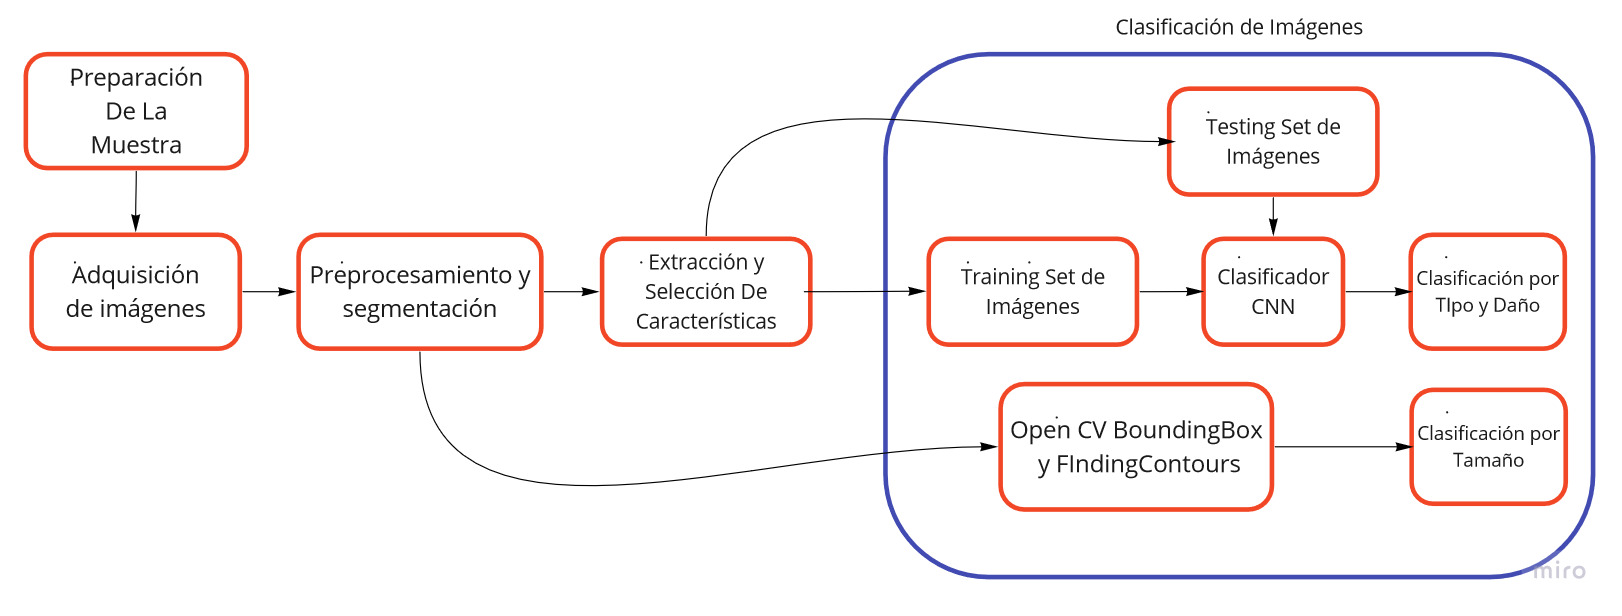
\includegraphics[scale=0.3]{Figs/FGGeneral.jpg}
	\caption{Arquitectura del Sistema de Clasificación}
	\label{fig:flujogeneral}
\end{figure}

El sistema propuesto para realizar la clasificación de tubérculos de papa en este documento, consiste desde la adquisición de muestras y creación de un dataset de tubérculos de papa hasta el diseño de un algoritmo de clasificación con Redes Neuronales utilizando la librería \textit{Pytorch} y la librería \textit{Open CV} de \textit{Python}. Será implementado en un prototipo de banda transportadora que permita el movimiento de los tubérculos de papa para ser clasificados mediante un microcontrolador y una cámara. Los sistemas de Visión Artificial que se destinan a realizar inspecciones visuales permiten que el proceso sea más eficiente si requieren alta velocidad, gran aumento en cantidad de producción y en funcionamiento las 24 horas del día o la repetibilidad de las medidas \cite{artificial2012aplicacion}.


\section{Preparación y Adquisición De Las Imágenes}

	Se preparó un total de 592 tubérculos de papá que manualamente fueron clasificados en tres categorías definidas. Las etiquetas de cada imagen se encuentran dentro del nombre de cada archivo, que corresponde al metadata de cada foto tomada. Definido de la siguiente manera:
	
	\begin{itemize}
		\item \textit{Tipo:} Pastusa o R12 $[0,1]$
		\item \textit{Daño:} Buena y Defectuosa $[0,1]$
		\item \textit{Tamaño:} Muy grande, Grande y Mediana $[0,1,2]$
		\item \textit{Numero de la Imágen} Etiqueta asignada por la cámara.
	\end{itemize}	
	
	Las fotos tomadas para la creacion del \textit{Dataset} poseen un tamaño de (3168, 4752) pixeles. Fueron tomadas con una cámara profesional \textit{Canon EOS 50D} que tiene 15.1 mega pixeles de resolución y se puede ajustar la sensibilidad ISO desde 100 a 3200. La cámara fue configurada con ISO-800 que corresponde al parámetro de sensibilidad del sensor de ruido de la cámara, una velocidad de obturación de $\frac{1}{640}$ segundos que corresponde al dispositivo que controla el tiempo en el que la luz incide sobre el sensor de la cámara y finalmente una apertura de diafragma de $F7.1$ que corresponde a la apertura del lente que deja pasar la luz \cite{Camara}, tener en cuenta que a mayor apertura de diafragma, menor luz se deja pasar. Se construyó una caja con iluminación fija \ref{fig:chamber} usando bombillos de luz blanca de 6500 Kelvin de temperatura de color para que la iluminación en todas las fotos tomadas fuera uniforme y la cámara fue fijada a un trípode para que la distancia de la cámara a la muestra de papa fuera siempre la misma en las 592 fotos.

	\begin{figure}[ht]
		\centering
		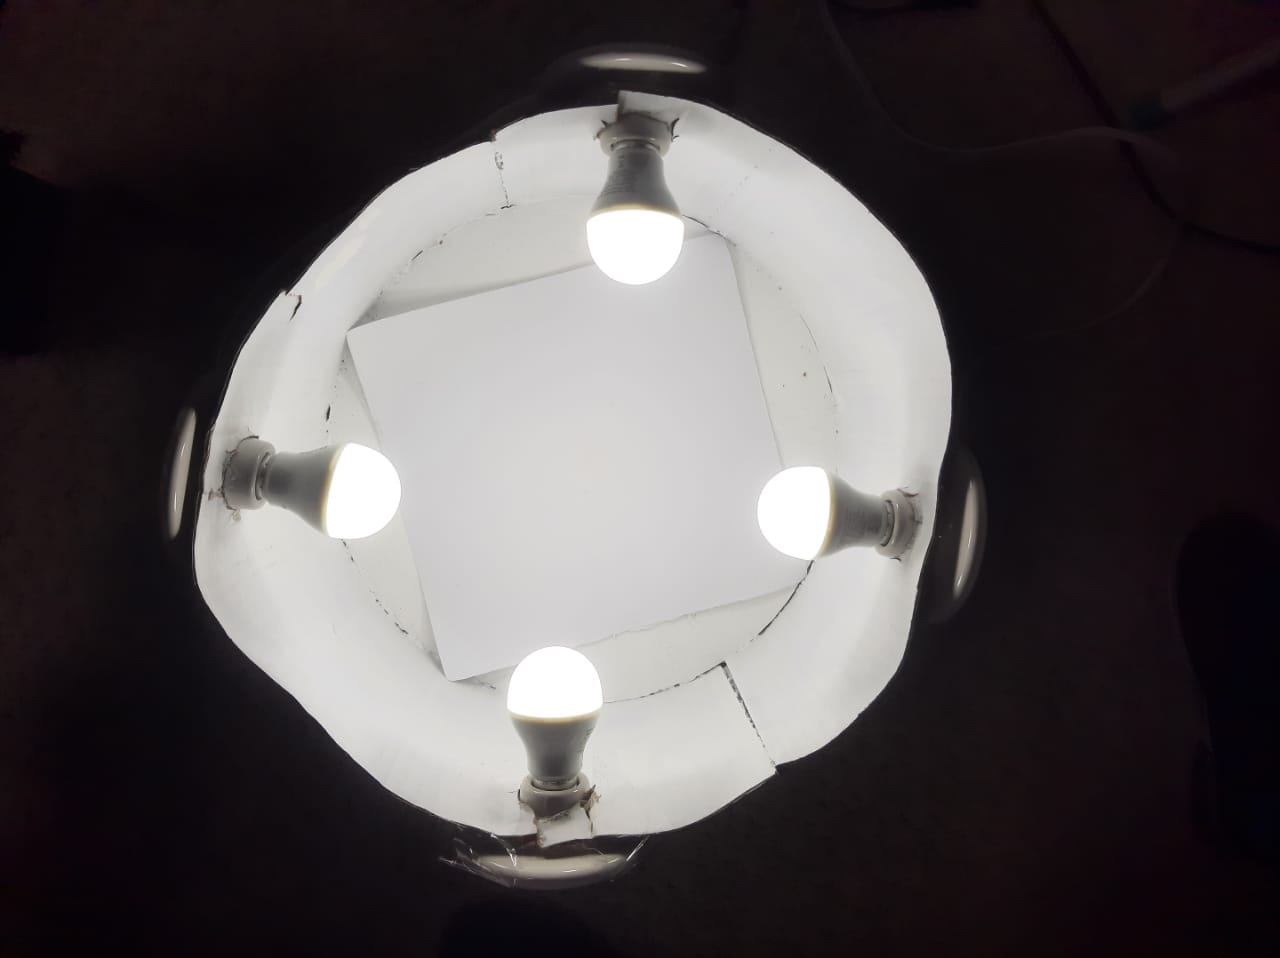
\includegraphics[scale=0.15]{Figs/Chamber.JPEG}
		\caption{Récamara Para la Toma de Fotos}
		\label{fig:chamber}
	\end{figure}
	
	Utilizando la librería \textit{Pandas} de \textit{Python}, se creó un \textit{Dataframe} que contiene el metadata de cada imágen. En la tabla \ref{table:metadata} podemos apreciar la distribución del \textit{MetaData} de las imagenes almacendas en el \textit{Dataset}, donde se toman cinco imágenes al azar como muestra. A partir de esta tabla se crea un archivo \textit{.CSV} donde se encuentra la informacion de las 592 imagenes.
	
	\begin{table}[ht]
		\centering
		\begin{tabular}{|c|c|c|c|}
			\hline
			Tipo & Daño & Tamaño & Filename \\
			\hline
			R12 & Defectuosa & Grande & 1\_1\_1\_075.JPG \\
			\hline
			PASTUSA & Buena & Grande & 0\_0\_1\_1973.JPG \\
			\hline
			R12 & Buena & Grande & 1\_0\_1\_2054.JPG \\
			\hline
			PASTUSA & Buena & Mediana & 0\_0\_2\_2042.JPG \\
			\hline
			PASTUSA & Buena & Grande & 0\_0\_1\_1955.JPG \\
			\hline
		\end{tabular}	
		\caption{MetaData de 5 Imágenes de Muestra}
		\label{table:metadata}
	\end{table}


	Una vez la información de cada imágen fue guardada en el archivo \textit{metadata.csv}, se agruparon las posibles combinaciones de las características de \textit{Tipo} y \textit{Daño} para definir las \textit{clases} dentro de la red neruonal. Para realizar este proceso se creó una condición dentro del \textit{Dataframe} que contiene el \textit{Metadata} para generar una columna adicional con la información de la tabla \ref{table:Clases}.	
	
	\begin{table}[ht]
		\centering
		\begin{tabular}{|c|c|c|c|c|}
			\hline
			PASTUSA & R12 & Buena & Defectuosa & Clase \\
			\hline
			X &  & X &  & CLASE 1 \\
			\hline
			X &  &  & X & CLASE 2 \\
			\hline
			& X & X &  & CLASE 3 \\
			\hline
			& X &  & X & CLASE 4 \\
			\hline
		\end{tabular}	
		\caption{Clases Definidas}
		\label{table:Clases}
	\end{table}	

De esta forma se definieron las $4 \ clases$ que serán entrenadas en la red neuronal para el posterior proceso de clasificación por visión artifical. 


\newpage
\section{Distribución del Dataset}
	  
	Para determinar la distribución total del dataset, con el uso de la librería \textit{Plotly} se crearon gráficas para determinar el porcentaje de imágenes pertenecientes cada característica definida en el \textit{Dataset}. La figura \ref{fig:distribuciontipo}
		
	\begin{figure}[ht]
		\centering
		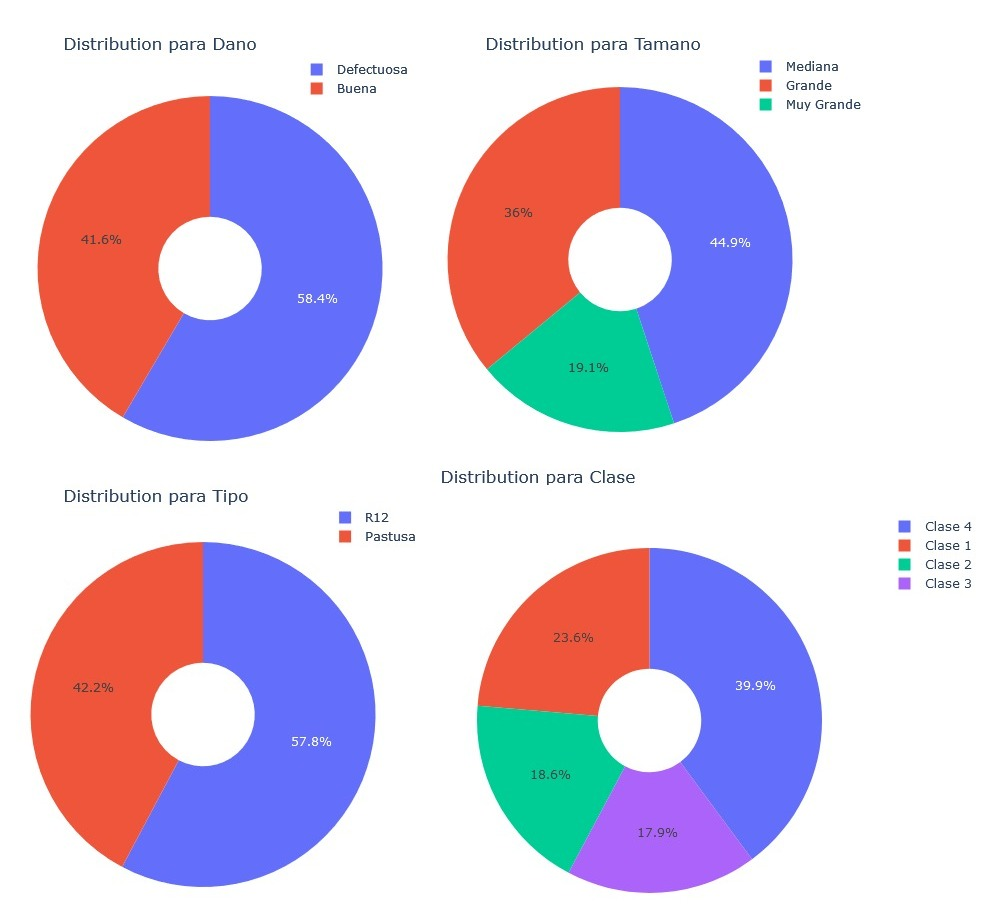
\includegraphics[scale=0.4]{Figs/Distribucion.jpg}
		\caption{Distribución del Dataset Según Sus Características Y Clases Definidas}
		\label{fig:distribuciontipo}
	\end{figure}

	Se definieron los \textit{Set's} de \textit{Train} y \textit{Test}, que fueron creados para el entrenamiento y validación de la red neuronal a partir del archivo \textit{metadata.csv} de la tabla \ref{table:metadata}. Se utilizó $80\%$ para \textit{Train} y $20\%$ para \textit{Test}. Se crearon los archivos \textit{train.csv} y \textit{test.csv} que contienen el \textit{metadata} y la dirección de las imágenes separadas en el respectivo $80\%$ y $20\%$.



\newpage
\chapter{Algoritmo de Clasificación}

	\section{Red Neuronal Artificial Convolucional}

	Se desarrolló una red neuronal artificial (\textit{CNN}) para clasificar las características de tipo y daño de los tubérculos de papas descritos en el \textit{Metadata} \ref{table:metadata}. La arquitectura general de una red artificial convolucional (\textit{CNN}) se muestra en la figura \ref{fig:cnnarchitecture} \cite{cnnarchitecture}. Se realizaron pruebas con las arquitecturas \textit{Alexnet}, \textit{Resnet18}, \textit{VGG11} y \textit{VGG19} y se implementó la optimización bayesiana en ciertos hiperparámetros de las arquitecturas existentes para mejorar los resultados. 
	
	\begin{figure}[ht]
		\centering
		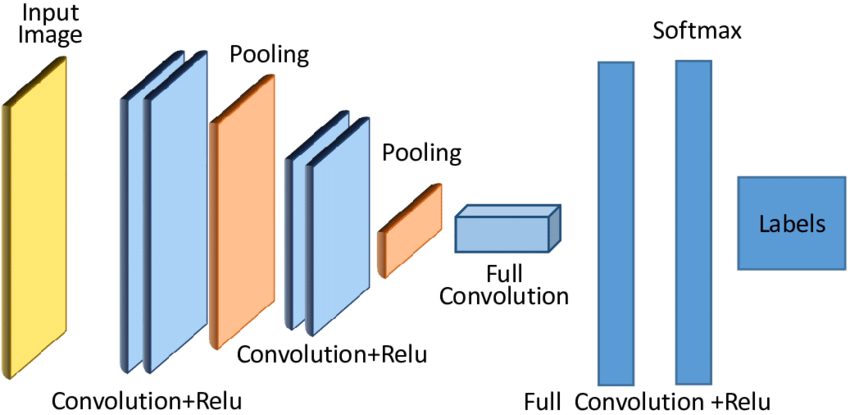
\includegraphics[scale=0.25]{Figs/A-generic-CNN-Architecture.png}
		\caption{Arquitectura General De Una CNN}
		\label{fig:cnnarchitecture}
	\end{figure}	
	
	El procedimiento realizado para desarrollar la red neuronal, descrito en la figura \ref{fig:procedimiento}, indica los pasos a seguir previo a implementar alguna de las arquitecturas. Cada item será descrito en las próximas secciones.  


	\begin{figure}[ht]
		\centering
		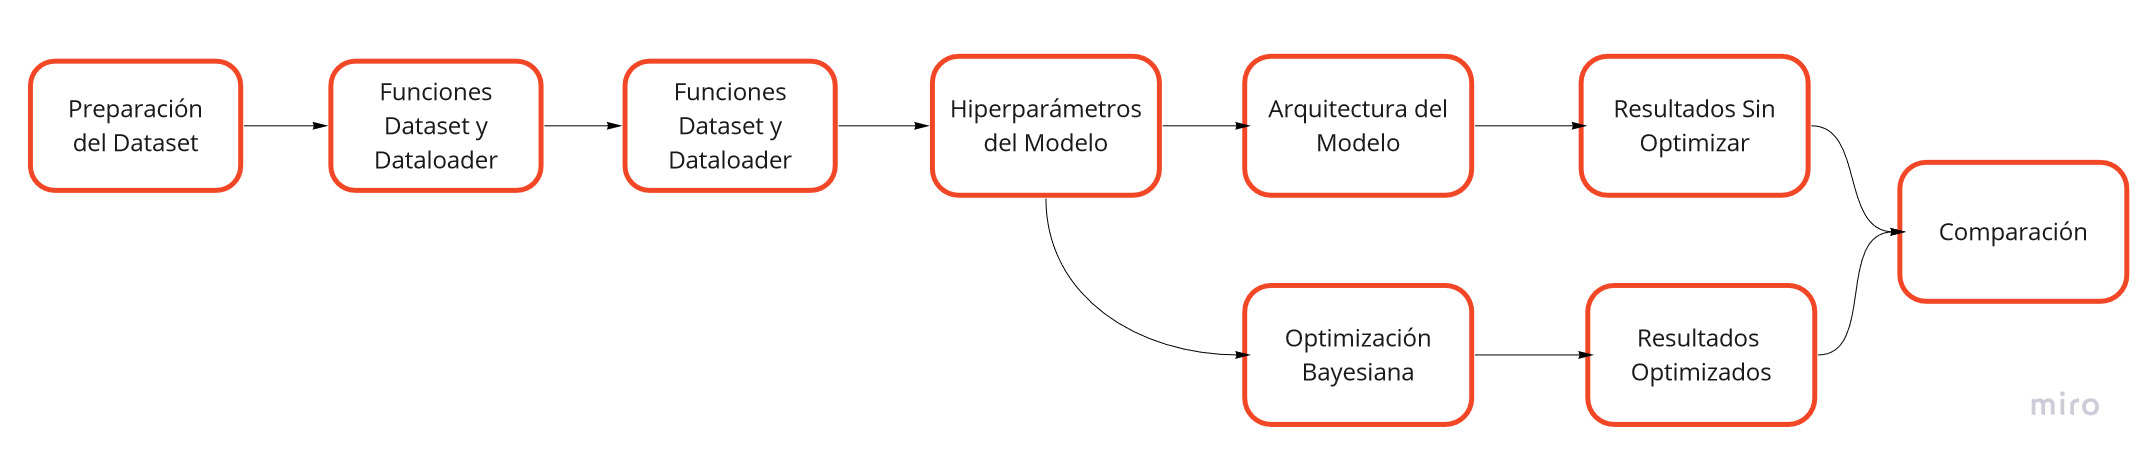
\includegraphics[scale=0.2]{Figs/procedimiento.jpg}
		\caption{Procedimiento Diseñado Para Implementar La \textit{CNN}}
		\label{fig:procedimiento}
	\end{figure}	


		\newpage
		\subsection{Preparación Del \textit{Dataset}}
			\subsubsection{DATA AUGMENTATION}

			El Data augmentation consiste en la transformación de los datos existentes para crear un \textit{dataset} con mayor cantidad de datos diferentes. El objetivo de esta herramienta es crear nuevos datos que puedan ser añadidos al conjunto ya existente y así contar con más muestras para un mejor desempeño del algoritmo. Además de esto tambien es implementado para reducir el \textit{overfitting} ya que al añadir más información al conjunto de entrenamineto se evita que el modelo se sobreajuste. \\


			El concepto Data Augmentation tiene relación con los procedimientos para edificar algoritmos iterativos de mejora o muestreo por medio de la introducción de datos no vigilados o cambiantes latentes. Para los algoritmos estocásticos, el procedimiento se popularizó en la literatura estadística por el algoritmo de incremento de datos de Tanner y Wong y en la literatura de física por el algoritmo de Swendsen y Wang para el muestreo de los modelos de Ising y Potts y sus generalizaciones; en la literatura de física, el Data Augmentation se conoce como el procedimiento de las cambiantes auxiliares. Generalmente, no obstante, la obra de esquemas de el Data augmentation es que den sitio a algoritmos básicos y rápidos, debido a que las tácticas famosas varían de una manera significativa con respecto a los modelos.\cite{van2001art}
					
			 
			\newpage
			\subsubsection{PREPROCESAMIENTO DE IMÁGENES}

			Usando el módulo \textit{torchvision.tranforms.compose()} de la librería \textit{Pytorch} se puede encadenar unas determinadas funciones que aplican diferentes tipos de filtros y transformaciones al \textit{Dataset}. De esta forma se puede crear la tarea de segmentación debido a que las transformaciones aumentan en consideración el tamaño original del \textit{Dataset}, facilitando así, la extracción de características de c ada imágen \cite{Pytorch}. Las tranformaciones disponibles en éste módulo se presentan a continuación:
			
			\begin{table}[ht]
				\centering
				\begin{tabular}{|p{4cm}|p{4cm}|p{4cm}|p{4cm}|}
					\hline
					Image Transform       & \multicolumn{1}{c|}{Use}                                                               & Image Transform       & \multicolumn{1}{c|}{Use}                                                                        \\ \hline
					CenterCrop            & Recorta la imágen en el centro                                                         & RandomResizedCrop     & Recorta una porción aleatoria de la imágen y la redimensiona a un tamaño determinado            \\ \hline
					ColorJitter           & Cambia aleatoriamente el brillo, el contraste, la saturación y el tono de una imágen   & RandomRotation        & Rota la imágen a un ángulo determinado                                                          \\ \hline
					FiverCrop              & Recorta la imágen en cuatro esquinas y el recorte central                              & RandomVerticalFlip    & Voltea verticalmente la imágen al azar con una probabilidad dada                                \\ \hline
					Grayscale             & Convierte la imágen en escala de grises                                                & Resize                & Redimensiona la imágen al tamaño dado                                                           \\ \hline
					Pad                   & Rellena la imágen en todos sus lados con el valor de "pad" dado                        & TenCrop               & Recorta la imagen dada en cuatro esquinas y el recorte central más la versión volteada de éstas \\ \hline
					RandomAffine          & Transformación afín aleatoria de la imagen manteniendo el centro invariante            & GaussianBlur          & Desenfoca la imágen con un filtro gausseano                                                                                                                                                     \\ \hline
				\end{tabular}
				\caption{Funciones de transformación de imágenes del módulo de \textit{Pytorch}}
				\label{table:Filters1}
			\end{table}
			
			En la tabla \ref{table:Filters1} se observa una parte de las transformaciones de imágenes disponibles en el módulo \textit{torchvision.tranforms.compose} de la librería \textit{Pytorch}. En el caso del \textit{Dataset} de papas creado, se deben tener en cuenta únicamente las transformaciones cuyo resultado sea relevante para la extracción de caractéristicas de la imágen, por ejemplo, eomo se explicó anteriormente, se va a clasificar el tubérculo de papá en tipo y daño con la red neuronal, por este motivo, el color es una característica que define si la papa pertenece a la clase \textit{R12} o \textit{Pastusa} y, en algunos casos, si se encuentra con algún tipo de daño, por este motivo, los filtros que transforman la imágen en escala de grises no son relevantes y podrían afectar el rendimiento del algoritmo.
		
			\begin{table}[ht]
				\centering
				\begin{tabular}{|p{4.5cm}|p{3.5cm}|p{3.8cm}|p{3.5cm}|}
					\hline
					Image Transform       & \multicolumn{1}{c|}{Use}                                                               & Image Transform       & \multicolumn{1}{c|}{Use}                                                \\ \hline
					Randomcrop            & Recorta la imágen aleatoriamente                                                       & RandomInvert          & Invierte los colores de la imágen de forma aleatoria                    \\ \hline
					RaandomGrayscale      & Convierte la imágen en escala de grises aleatoriamente                                 & RandomPosterize       & Reduce el número de bits de cada canal de laa imágen de forma aleatoria \\ \hline
					RandomHorizontalFlip  & Voltea horizontalmente la imágen al azar con una probabilidad dada                     & RandomSolarize        & Invierte aleatoriamente el valor de los pixeles por encima de un umbral \\ \hline
					RandomPerspective     & Realiza una transformación de perspectiva aleatoria de la imagén                       & RandomAutocontrast    & Autocontraste de los píxeles de la imagen dada aleatoriamente           \\ \hline
					RandomAdjustSharpness & Ajusta la nitidez de la imágen de forma aleatoria                                      & RandomEqualize        & Equaliza el histograma de la imágen dada aleatoriamente                 \\ \hline
					RandomApply           & Aplicar aleatoriamente una lista de transformaciones con una probabilidad determinada. & \multicolumn{1}{l|}{} &                                                                         \\ \hline
				\end{tabular}
				\label{table:filters2}
				\caption{Funciones de transformación de imágenes del módulo de \textit{Pytorch}}
			\end{table}

			De igual forma, en la tabla \ref{table:filters2}, se observan algunos filtros como recortes en la imágen, rotaciones, cambios de perspectiva, cambios en la nitidez y contraste de la imágen. Se escogieron los filtros considerados mejores para el caso del \textit{Dataset} de tubérculos de papa creado en este documento. 
			
			
			
			\newpage
			Los filtros que se utilizaron en el desarrollo del algoritmo de clasificación, teniendo en cuando aquellas transformaciones que podrían afectar el rendimiento del algoritmo fueron:
			
			\begin{itemize}
				\item Resize
				\item ColorJitter
				\item RandomRotation
				\item GaussianBlur
				\item RandomPerspective
				\item RandomAdjustSharpness
			\end{itemize}

			Como se está utilizando la librería \textit{Pythorch}, las imágenes deben ingresar en formato \textit{Tensor}, que convierte los valores de los píxeles de una imágen \textit{PIL} estándar con un rango de $[0, 255]$  a un tensor decimal de \textit{Pythorch} con valores en un rango de con valores $[0.0, 1.0]$ de la forma  $(C, H, W)$, siendo C el número de canales de la imágen (1 si es en escala de grises, 3 si es \textit{RGB}), $H$ y $W$ el tamaño de la imágen. \\
			
			Una vez la imágen está en formato \textit{PyTorch FloatTensor}, se decidió utilizar la función \textit{torchvision.tranforms.normalize()} para normalizar las imágenes. La normalización de una imágen consiste en modificar los valores del tensor, que se encuentran entre $[0.0, 1.0]$ para que el promedio y la desviación estándar sean $0$ y $1$ respectivamente. Para hacer esto se utiliza la ecuación \ref{eq:normalize} \cite{Pytorch}
			
			\begin{equation}
				{output[Channel]=\frac{Input[Channel]-Mean[Channel]}{std[Channel]}}
				\label{eq:normalize}
			\end{equation}

			La normalización se utiliza debido a que ayuda a los datos a estar definidos dentro de un rango y reducir la asimetría entre ellos, lo que permite un aprendizaje más rápido. Se diseñó una función en \textit{Python} que calcula el promedio y al desviación estándar para \textit{Trainset} y para el \textit{Testset}. De esta forma se garantiza que la normalización sea correcta en el total del \textit{Dataset}. Los valores obtenidos para el \textit{Trainset} \ref{eq:meanstd1} y el \textit{Testset} \ref{eq:meanstd2} respectivamente.
			
			\begin{equation}				{mean = [0.7467, 0.7389, 0.7432] \hspace*{1cm}  std  = [0.1288, 0.1633, 0.2045]}
				\label{eq:meanstd1}
			\end{equation}


			\begin{equation}
				{mean = [0.7507, 0.7430, 0.7486] \hspace*{1cm}  std  = [0.1265, 0.1609, 0.2012]}
				\label{eq:meanstd2}
			\end{equation}


			La figura \ref{fig:agumentation} enseña una matriz de imágenes como parte del \textit{Trainset}, que muestra las transformaciones hechas al $80\%$ de las imágenes del \textit{Dataset} y la clase a la que pertenece \ref{table:Clases}, verificando así que las funciones creadas están enlanzando correcta la imágen con su respectiva clase y aplicando de forma correcta las transformaciones.

			\newpage
			\begin{figure}[ht]
				\centering
				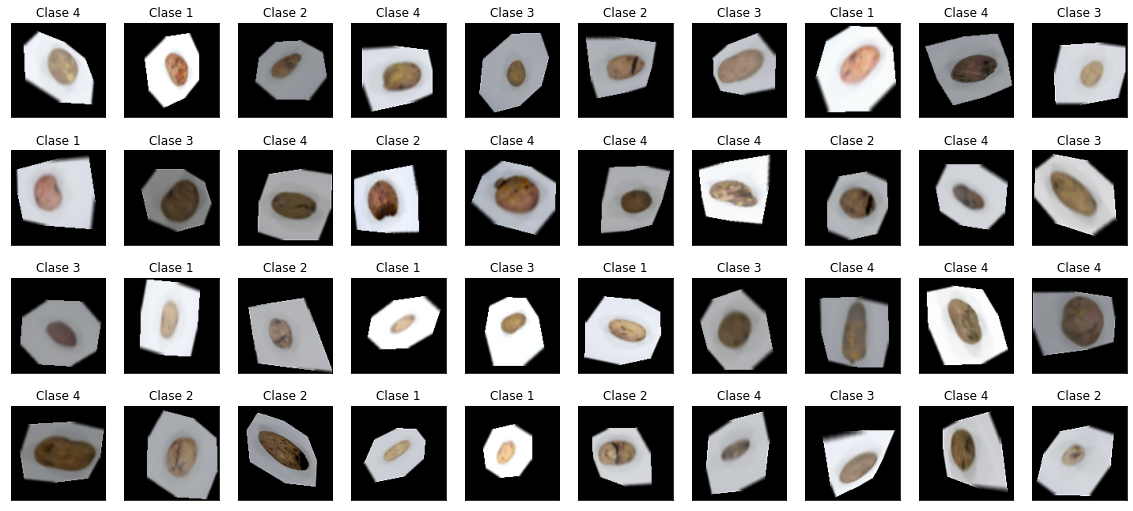
\includegraphics[scale=0.4]{Figs/augmentation.png}
				\caption{Matriz de Imagenes Con Transformaciones Aplicadas}
				\label{fig:agumentation}
			\end{figure}	

		\subsection{Funciones PotatoDataset y DataLoader}
		
		
			\subsubsection{FUNCIÓN POTATODATASET}
			
			Se creó una clase (\textit{Python Class Object Constructor}) con el nombre de \textit{AttributesDataset()} que se encarga de leer el \textit{Metadata}  de cada imágen y convertirlo en \textit{labelID} en la tabla \ref{table:metadata} se muestra como son ingresadas las imágenes en el algoritmo, sin embargo, las características deben ser ingresadas como \textit{labelID}, es decir, el label Pastusa corresponde al ID 0 en la categoría de Tipo. Este diccionario se presenta a continuación:			
	
			\begin{itemize}
				\item Tipo: ${'Pastusa': 0, 'R12': 1}$
				\item Daño: ${'Buena': 0, 'Defectuosa': 1}$
				\item Tamaño: ${'Muy Grande': 0, 'Grande': 1, 'Mediana': 2}$
			\end{itemize}

			En la red neuronal únicamente se utilizaron \textit{labels} y \textit{labelID} de tipo y daño para definir las clases \ref{table:Clases}. La función \textit{Dataset} de \textit{Python} realiza el proceso cargar y relacionar relacionar cada imágen con su respectivo \textit{label} para \textit{Dataset's} que se encuentran organizados dentro de carpetas jerarquicamente. El \textit{Dataset} creado en éste documento no se encuentra organizado de esta manera, sino que la organización jerarquica que define las clases se encuentra dentro del \textit{metadata} en el nombre de cada imágen \ref{table:metadata}, debido esto es que se desarrolló una función que cargara y relacionara de la misma manera que lo hace la función integrada de \textit{Pythorch}. Esta función fue llamada \textit{PotatoDataset()} que utiliza los \textit{labelID} generados por la función \textit{AttributesDataset()} y carga cada imágen relacionada con sus \textit{labelID}. Como se desarrolló la función, de igual forma debe ser capas de aplicar las transformaciones a cada imágen. El objeto regresa las 592 imágenes cargadas en \textit{Python} cada una relacionada con su respectivo \textit{labelID} y \textit{label} y con una transformación o múltiples aplicadas. Esta función desarrollada cuenta con los mismos atributos iterables que poseen los \textit{dataset's} creados a partir de la función integrada en \textit{Pytorch}.			
			
		
			\subsubsection{FUNCIÓN DATALOADER}			
						
			Generalmente una vez se finaliza el proceso de cargar las imágenes utilizando la función \textit{DataSet} de \textit{Pytorch}, se procede a utilizar la función \textit{DataLoader} para generar múltiples lotes de imágenes a partir de las transformaciones utilizadas. La función \textit{DataLoader()} de \textit{Pytorch} es implementada para realizar la importación de datos a gran escala. Para el uso de esta función se debe tener en cuenta que el argumento más importante será el \textit{dataset} que fue generado por el objeto \textit{PotatoDataset()}. \\
			
			Según como se explico en el apartado anterior, se generó un \textit{dataset} del tipo \textit{iterable-style Datsets}, lo que permite utilizar la función integrada \textit{DataLoader()} de \textit{Pytorch}. El \textit{DataLoader} permite la agrupación automática de muestras de datos individuales obtenidas en los \textit{Batch's} mediante argumentos. Los \textit{DataLoader's} cuentan con una gran catidad de argumentos que ayudan para que la carga de datos sea más eficiente \cite{Pytorch}. Es por esta razón que para la ejecución de este dataloader se implementarón los siguientes parametros:
			
			\begin{table}[ht]
				\centering
				\begin{tabular}{|p{3cm}|p{8cm}|}
					\hline
					FUNCIÓN & DESCRIPCIÓN \\ 
					\hline
					Batch size & Cuántas muestras por Batch hay que cargar (Default: 1)\\
					\hline
					Shuffle & Se establece en TRUE para que los datos se reorganicen en cada época (Default: FALSE)  \\
					\hline
					Num workers & Cuántos subprocesos se utilizarán para la carga de datos. 0 significa que los datos se cargarán en el proceso principal. (Default: 0)\\
					\hline
				\end{tabular}	
				\caption{Argumentos para el Dataloader}
				\label{table:Argumentos}
			\end{table}
		
		Los argumentos explicados en la tabla anterior fueron establecidos de la siguiente forma:
		
		\begin{itemize}
			\item $Batch \ Size = 40$
			\item $Shuffle = True$
			\item $Num \ workers = 0$
		\end{itemize}

		Esto con el obejtivo de que el Dataloader cargue 40 muestras por época y tome otras 40 diferentes para la siguiente época y asi sucesivamete hasta terminar todas las epocas estrablecidas.  
		
		
		
			
		
		\subsection{Hiperparámetros Del Modelo}
			\subsubsection{FUNCIÓN DE PÉRDIDAS}
			
			
			incluir parte matematica?
			\subsubsection{\MakeUppercase{Optimizador}}
			
			
			momentum y learning rate
			\subsubsection{\MakeUppercase{Backward pero otro nombre}}
			
			
		\subsection{Optimización Bayesiana}	
			
			
		\subsection{Arquitectura del modelo}
			\subsubsection{\MakeUppercase{Modelo preentrenado ALEXNET}}
			El modelo AlexNet fue implementado en el año 2012 en el desafio de reconocimiento visual a gran escala Imaget. Este modelo tuvo un resultado tan satisfactorio que los modelos de aprendizaje profundo se convirtieron en la referencia para la investigación y desarrollo en los principales sectores de la industria. \cite{Pytorch}
			\\
			El modelo de AlexNet toma una imagen de entrada de tamaño 227*227(*3 canales de color) y aplica una convolución de tamaño 11*11 (con 96 núcleos/canales de salida) con un paso de 4. La salida de la convolución es una Imagen de 56*56*96 que luego pasa por otras capas hasta que llega a la capa softmax para su clasificación como se muestra en la siguiente imagen:
			
			\begin{figure}[ht]
				\centering
				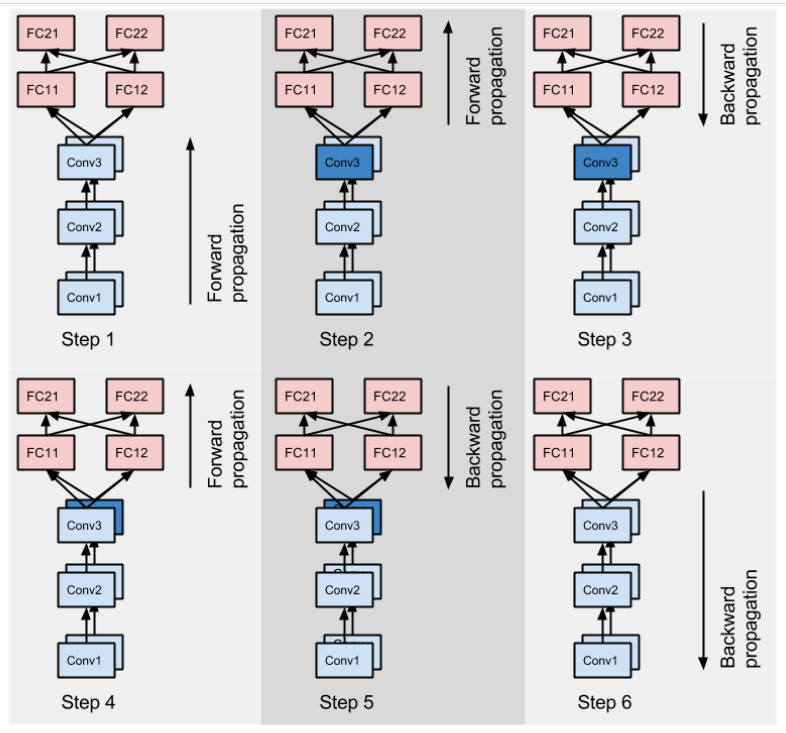
\includegraphics[scale=0.4]{Figs/5.png}
				\caption{Modelo AlexNet}
				\label{fig:AlexNet}
			\end{figure}
		
			Una vez conocida la estructura del modelo procedemos con la implementación, en la cual se siguieron una serie de pasos para la construcción del modelo clasificadorlos cuales son:
			
			\begin{enumerate}
				\item \textbf{CARGAR BIBILIOTECAS IMPORTANTES:} 
				\\
				Se llaman las bibliotecas importantes para la ejecución del modelo entre estas tenemos torch para pytorch...
				\item \textbf{PREPARACIÓN CONJUNTO DE DATOS:} 
				\\
				La preparación del conjunto de datos es una etapa de importación en la creación y ejecución del algoritmo de red neuronal o también conocida como preprocesamiento de imagenes.
				\item\textbf{CONSTRUCCIÓN DEL MODELO}
				\\
				En esta parte se convierte la arquitectura de AlexNet presentada en la imagen ... en código, para poder usarla más adelante en la clasificación.
				Además en este paso se definen los valores de el maxpooling, el padding y el número de convoluciones que tendra la red neuronal.
				\item\textbf{FORMACIÓN DEL MODELO}
				\\
				Durante el entrenamiento de la red AlexNet (entrenamiento durante ... epochs) se obtuvo una precisión de validación promedio del ..., como se muestra en la siguiente imagen:
				\item \textbf{PRUEBA DEL MODELO}
				\\
				En este paso se comprueba la eficiencia del modelo usando el dataset de validación, donde encontramos que la red AlexNet pudo predecir correctamente ... de ... imagenes de papas tanto defectuosas como en buen estado y reconociendo tambien el tamaño al que pertenecen ya sea grande, mediana o pequeña 
			\end{enumerate} 
			
			\subsubsection{\MakeUppercase{Modelo preentrenado RESNET18}}
			Una red residual, o ResNet para abreviar, es una red neuronal artificial que ayuda a construir una red neuronal más profunda mediante la utilización de conexiones de salto o accesos directos para saltar sobre algunas capas. Verá cómo la omisión ayuda a crear capas de red más profundas sin caer en el problema de los gradientes que se desvanecen.
		
			Hay diferentes versiones de ResNet, incluidas ResNet-18, ResNet-34, ResNet-50, etc. Los números denotan capas, aunque la arquitectura es la misma.
			
			Los profesionales implementan modelos clásicos de redes neuronales residuales con saltos de 2 o 3 capas que tienen dentro normalización por lotes y no linealidad entre ellas. Los científicos de los datos además aprovechan una matriz de peso extra para aprender los pesos de los saltos en algunas ocasiones. El concepto usado para explicar este fenómeno es “Redes de autopistas”. Los modelos que consisten en diversos saltos paralelos son “Densenets”. Las redes no residuales además tienen la posibilidad de nombrar redes primordiales una vez que se habla de redes neuronales residuales.
			
			\begin{figure}[ht]
				\centering
				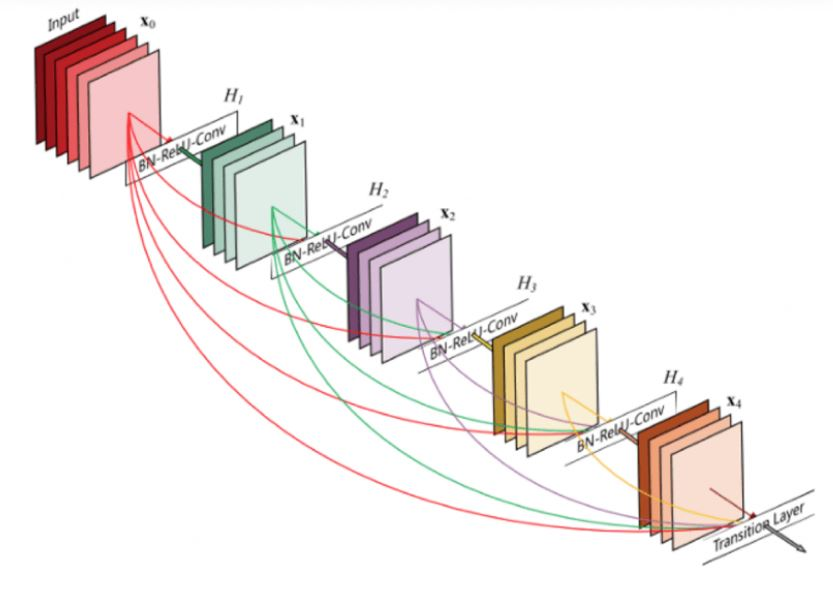
\includegraphics[scale=0.6]{Figs/6.jpg}
				\caption{Modelo ResNet18}
				\label{fig:ResNet18}
			\end{figure}
			\subsubsection{\MakeUppercase{Modelo preentrenado VGG19}}
			\subsubsection{\MakeUppercase{Modelo preentrenado VGG11}}
			\subsubsection{\MakeUppercase{Comparación de arquitecturas}}
		
	\section{Clasificación de tamaño}
	
\chapter{Prototipo}
	

	















